\subsection{Partition Results:}

\subsubsection{Worst case:}

First test for {\bfseries\itshape Partition}. The program will plot the {\bfseries\itshape time} that the algorithm takes to finish his process with a list sorted in decreasing order of length {\bfseries\itshape n = 6}. \hfill \break

{\bfseries\itshape\color{armygreen}{Observation:}} {\itshape\color{armygreen}{We are going to analyze the worst case when the list it's sorted in decreasing order.}} \hfill \break

\begin{figure}[H]
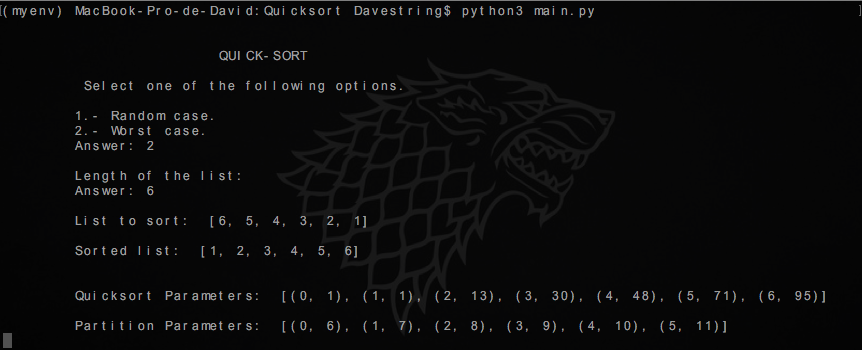
\includegraphics[scale=.54]{pt1.png}
\centering \linebreak \linebreak Figure 4.2.1.0: Testing Partition with a list of length n = 6.
\end{figure} \hfill 

\begin{multicols}{2}
\begin{figure}[H]
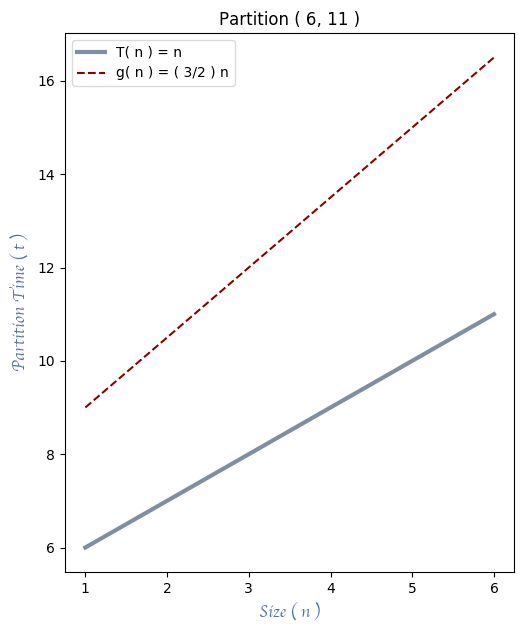
\includegraphics[scale=.5]{pp1.png}
\centering \linebreak \linebreak Figure 4.2.1.1: Graph for Figure 4.2.1.0.
\end{figure} \hfill

\begin{center}
\begin{itemize}

\end{itemize}
{\Large
\begin{tabular}[.5cm]{ c c c }
\toprule
Length ( n ) & Time ( t ) \\
\midrule
0 & 6 \\
\cmidrule {1-2}
1 & 7 \\
\cmidrule {1-2}
2 & 8 \\
\cmidrule {1-2}
3 & 9 \\
\cmidrule {1-2}
4 & 10 \\
\cmidrule {1-2}
5 & 11 \\
\cmidrule {1-2}
6 & 12 \\
\bottomrule
\linebreak
\end{tabular}}
\linebreak \linebreak Table 5: Plot point for Figure 4.2.1.1.
\end{center}
\end{multicols}

\pagebreak

Second test for {\bfseries\itshape Partition}. The program will plot the {\bfseries\itshape time} that the algorithm takes to finish his process with a list sorted in decreasing order of length {\bfseries\itshape n = 20}. \hfill \break

\begin{figure}[H]
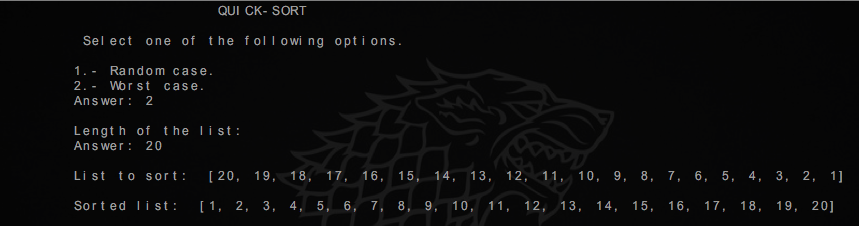
\includegraphics[scale=.54]{pt2.png}
\centering \linebreak \linebreak Figure 4.2.1.2: Testing Partition with a list of length n = 20.
\end{figure} \hfill

\begin{multicols}{2}
\begin{figure}[H]
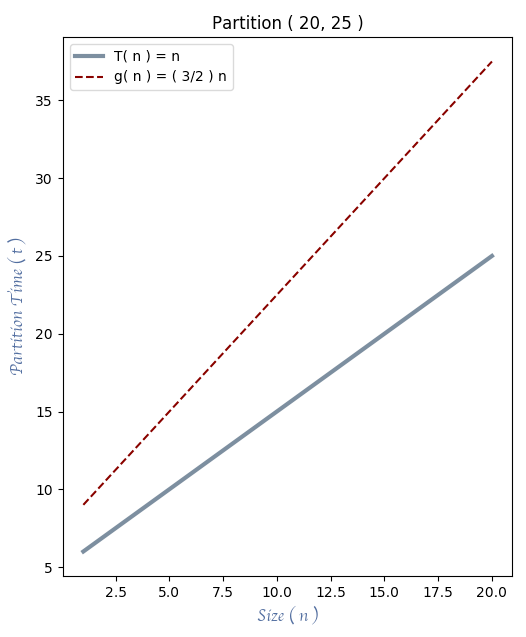
\includegraphics[scale=.5]{pp2.png}
\centering \linebreak \linebreak Figure 4.2.1.3: Graph for Figure 4.2.1.2.
\end{figure}

\begin{center}
\begin{itemize}

\end{itemize}
\begin{tabular}[.5cm]{ c c c }
\toprule
Length ( n ) & Time ( t ) \\
\midrule
0 & 6 \\
\cmidrule {1-2}
1 & 7 \\
\cmidrule {1-2}
2 & 8 \\
\cmidrule {1-2}
3 & 9 \\
\cmidrule {1-2}
4 & 10 \\
\cmidrule {1-2}
5 & 11 \\
\cmidrule {1-2}
6 & 12 \\
\cmidrule {1-2}
7 & 13 \\
\cmidrule {1-2}
8 & 14 \\
\cmidrule {1-2}
9 & 15 \\
\cmidrule {1-2}
10 & 16 \\
\cmidrule {1-2}
11 & 17 \\
\cmidrule {1-2}
12 & 18 \\
\cmidrule {1-2}
13 & 19 \\
\cmidrule {1-2}
14 & 20 \\
\cmidrule {1-2}
15 & 21 \\
\cmidrule {1-2}
16 & 22 \\
\cmidrule {1-2}
17 & 23 \\
\cmidrule {1-2}
18 & 24 \\
\cmidrule {1-2}
19 & 25 \\
\cmidrule {1-2}
20 & 26 \\
\bottomrule
\linebreak
\end{tabular}
\linebreak \linebreak Table 6: Plot point for Figure 4.2.1.3.
\end{center}
\end{multicols} \hfill

{\bfseries\itshape\color{armygreen}{Observation:}} {\itshape\color{armygreen}{The {\bfseries red} graph represents our proposed function for the worst case of {\bfseries Partition} and the {\bfseries blue} one it's the temporal complexity.}} \hfill \break

{\bfseries\itshape\color{armygreen}{Observation:}} {\itshape\color{armygreen}{The function proposed is: {\bfseries g( n ) = ( 3/2 ) n}. }} \hfill \break

\pagebreak

\subsubsection{Random case:}

Third test for {\bfseries\itshape Partition}. The program will plot the {\bfseries\itshape time} that the algorithm takes to finish his process with a list of random elements of length {\bfseries\itshape n = 10}. \hfill \break

\begin{figure}[H]
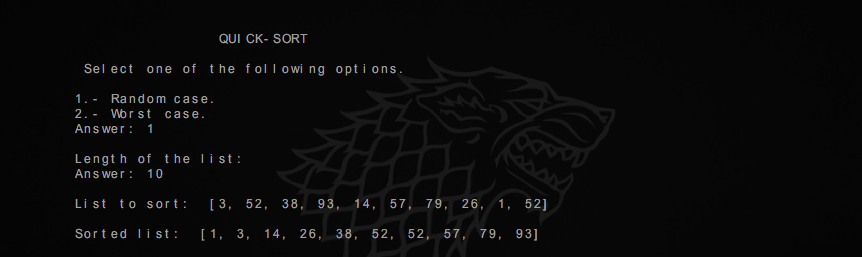
\includegraphics[scale=.54]{t3.png}
\centering \linebreak \linebreak Figure 4.2.2.0: Testing Partition with a list of length n = 10.
\end{figure} \hfill 

\begin{multicols}{2}
\begin{figure}[H]
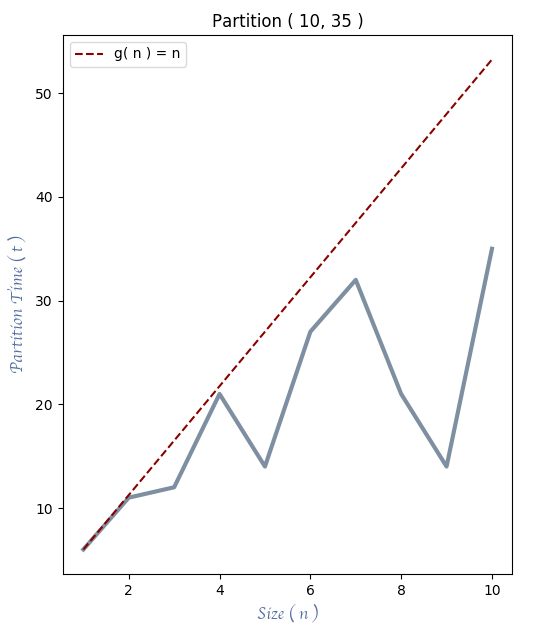
\includegraphics[scale=.5]{pp3.png}
\centering \linebreak \linebreak Figure 4.2.2.1: Graph for Figure 4.2.2.0.
\end{figure} \hfill

\begin{center}
\begin{tabular}[.5cm]{ c c c }
\toprule
Length ( n ) & Time ( t ) \\
\midrule
0 & 6 \\
\cmidrule {1-2}
1 & 11 \\
\cmidrule {1-2}
2 & 12 \\
\cmidrule {1-2}
3 & 21 \\
\cmidrule {1-2}
4 & 14 \\
\cmidrule {1-2}
5 & 27 \\
\cmidrule {1-2}
6 & 32 \\
\cmidrule {1-2}
7 & 21 \\
\cmidrule {1-2}
8 & 14 \\
\cmidrule {1-2}
9 & 35 \\
\bottomrule
\linebreak
\end{tabular}
\linebreak \linebreak Table 7: Plot point for Figure 4.2.2.1.
\end{center}
\end{multicols}

\pagebreak

Fourth test for {\bfseries\itshape Partition}. The program will plot the {\bfseries\itshape time} that the algorithm takes to finish his process with a list of random elements of length {\bfseries\itshape n = 15}. \hfill \break

\begin{figure}[H]
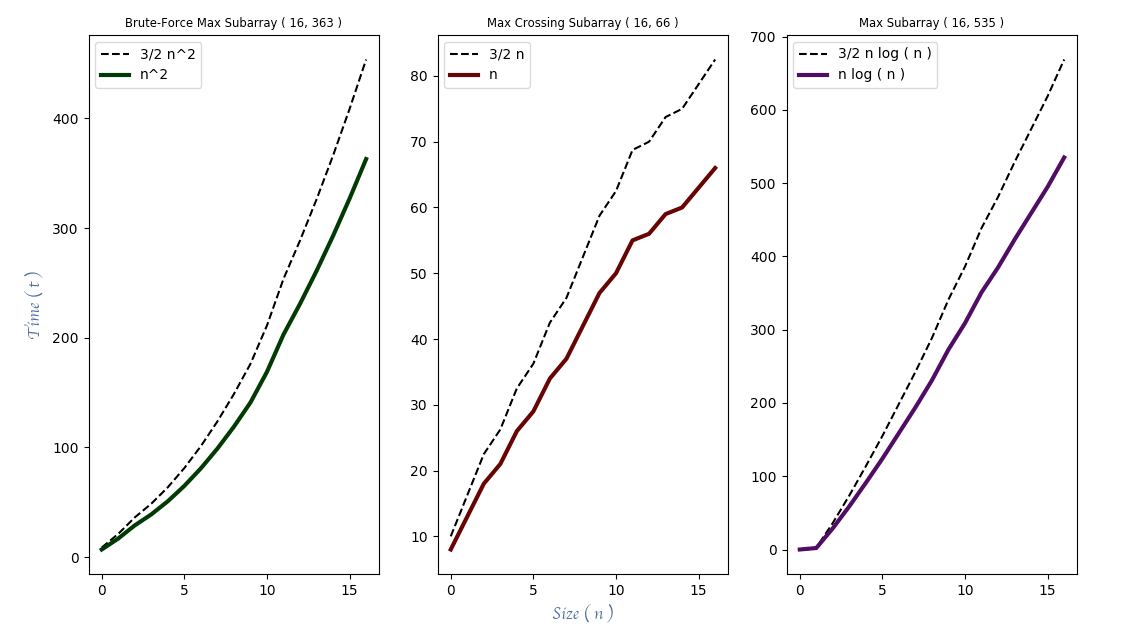
\includegraphics[scale=.54]{t4.png}
\centering \linebreak \linebreak Figure 4.2.2.2: Testing Partition with a list of length n = 15.
\end{figure} \hfill 

\begin{multicols}{2}
\begin{figure}[H]
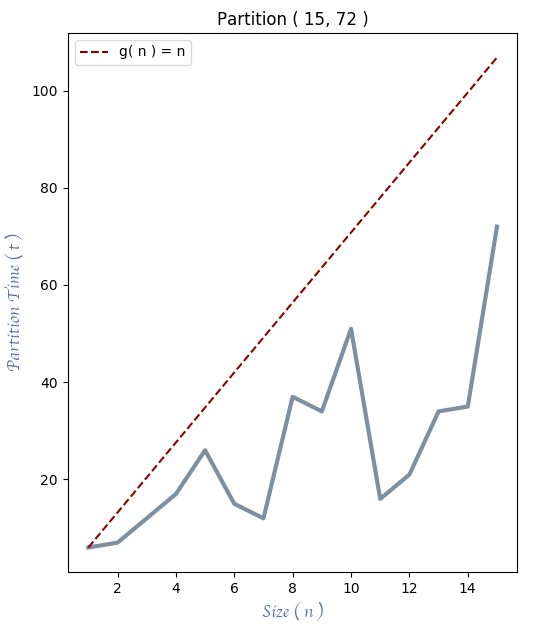
\includegraphics[scale=.5]{pp4.png}
\centering \linebreak \linebreak Figure 4.2.2.3: Graph for Figure 4.2.2.2.
\end{figure} \hfill

\begin{center}
\begin{tabular}[.5cm]{ c c c }
\toprule
Length ( n ) & Time ( t ) \\
\midrule
0 & 6 \\
\cmidrule {1-2}
1 & 7 \\
\cmidrule {1-2}
2 & 12 \\
\cmidrule {1-2}
3 & 17 \\
\cmidrule {1-2}
4 & 26 \\
\cmidrule {1-2}
5 & 15 \\
\cmidrule {1-2}
6 & 12 \\
\cmidrule {1-2}
7 & 37 \\
\cmidrule {1-2}
8 & 34 \\
\cmidrule {1-2}
9 & 51 \\
\cmidrule {1-2}
10 & 16 \\
\cmidrule {1-2}
11 & 21 \\
\cmidrule {1-2}
12 & 34 \\
\cmidrule {1-2}
13 & 35 \\
\cmidrule {1-2}
14 & 72 \\
\bottomrule
\linebreak
\end{tabular}
\linebreak \linebreak Table 8: Plot point for Figure 4.2.2.3.
\end{center}
\end{multicols} \hfill \break 

{\bfseries\itshape\color{armygreen}{Observation:}} {\itshape\color{armygreen}{The {\bfseries red} graph represents our proposed function for any other case of {\bfseries Partition} and the {\bfseries blue} one it's the temporal complexity.}} \hfill \break

{\bfseries\itshape\color{armygreen}{Observation:}} {\itshape\color{armygreen}{The function proposed is: {\bfseries g( n ) = ( 3/2 ) n}. }} \hfill \break

\pagebreak